% Нодири Хисравхон, P3131, 26.11.2022: 03:22, Begin lab 5 LaTeX, Kill me.
% Var: 26 -> 1972 / 6
% https://kvant.ras.ru/1972/06/p56.htm / https://kvant.ras.ru/1972/06/o_sistemah_fizicheskih_edinic.htm

\documentclass{memoir}

\usepackage[utf8]{inputenc}
\usepackage[russian]{babel}
\usepackage{multicol}
\usepackage[14pt]{extsizes}
\usepackage[left=10mm, top=-1mm, right=10mm, bottom=10mm, nohead, nofoot]{geometry}
\usepackage{graphicx}
\usepackage[usenames]{color}
\usepackage[most]{tcolorbox}
\usepackage{colortbl}
\usepackage{fancyhdr}
\usepackage[document]{ragged2e}
\usepackage{afterpage}

\graphicspath{{pictures/}}
\setlength\columnsep{60pt}
\pagestyle{fancy}
\fancyhf{}
\DeclareGraphicsExtensions{.png}
\fancyfoot[L]{56}

\begin{document}
\begin{multicols}{2}
\begin{small}
\begin{justify}

\parindent0pt
виде\linebreak
\parindent60pt

$\varphi$ = $\frac{q}{r} + c$, \indent (6)\linebreak

\parindent0pt

где c - произвольная постоянная,\linebreak
можно с помощью (2) получить закон\linebreak
Кулона. Это и будет означать, что\linebreak
формула (6), которая приводится без\linebreak
доказательств в школьном курсе фи-\linebreak
зики, действительно определяет по-\linebreak
тенциал точечного заряда в системе\linebreak
СГСЭ.\linebreak


\parindent20pt
В самом деле, пусть точечный\linebreak
заряд $q_2$ смещается в поле другого\linebreak
точечного заряда $q_1$ на очень малый\linebreak
отрезок r. Тогда, согласно форму-\linebreak
лам (2) и (6), \\\\
$\Delta A$ = - $q_2$($\varphi$$_2$ - $\varphi$$_2$) = -$q_2$$q_1$ $\times$ \\
\parindent60pt
\indent $\times$($\frac{1}{r + r} - \frac{1}{\Delta r}$) = $\frac{q_1 q_2 \Delta r}{r^2 + r \Delta r}$. \\\
\parindent20pt
\indent Так как $\Delta r$ мало, то $r^2$ $\gg$ r$\Delta$r и \\
\parindent45pt
\indent $\Delta A$ = $F \Delta r$ = $\frac{q_1 q_2}{r^2} \Delta r .$ \\

\parindent0pt
Следовательно, сила $F$ равна $\frac{q_1 q_2}{r^2},$\linebreak
а это и есть закон Кулона. Значит,\linebreak
формула (6) справедлива. \\
\parindent20pt

\indent Подобно тому как напряженность\linebreak
поля сферически симметрично заря-\linebreak
женного шара совпадает с напряжен-\linebreak
ностью точечного заряда, потенциал\linebreak
заряженного шара (вне шара) так-\linebreak
же определяется формулой (6). В\linebreak
системе СИ\\

	\parindent50pt
\indent $\varphi$ = $\frac{q}{4 \pi \varepsilon_2 \varepsilon r} + c$, \hfill (7) \\\\
если шар находится в однородном\linebreak
диэлектрике с диэлектрической про-\linebreak
ницательностью $\varepsilon$. \\
\parindent20pt
\indent Для решения задач достаточно\linebreak
хорошо представлять себе физиче-\linebreak
ский смысл основных форму. Кро-\linebreak
ме того, часто приходится использо-\linebreak
вать простые, но очень важные по-\linebreak
ложения: работа электростатиче-\linebreak
ского поля на замкнутом пути равна\linebreak
нулю и все точки проводника в элект-\linebreak
ростатике имеют один и тот же по-\linebreak
тенциал. \\
\indent З а д а ч а 1. Может ли сущест-\linebreak
вовать электрическое поле, на-\linebreak
пряженность которого не меняется\linebreak
в направлении $x$ и возрастает в на-\linebreak
правлении $y$ (рис. 1)? \\

\indent Р е ш е н и е. Не может, так как\linebreak
в таком поле работа при перемеще-\linebreak
нии заряда по замкнутому контуру \\

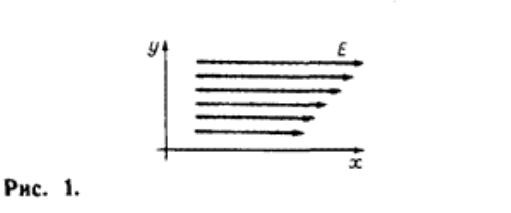
\includegraphics[scale=0.45]{pic1.png}\linebreak
(например, прямоугольному со сто-\linebreak
ронами, параллельными $x$ и $y$) от-\linebreak
лична от нуля. \\

\indent З а д а ч а 2. К внутренней стен-\linebreak
ке изолированного от земли электро-\linebreak
метра прикреплен металлический\linebreak
листочек (рис. 2). Стержень и кор-\linebreak
пус электрометра соеденили прово-\linebreak
дом и после этого сообщили корпусу\linebreak
электрометра некоторый заряд. От-\linebreak
клонятся ли при этом листочки элект-\linebreak
рометра? Что произойдет с листоч-\linebreak
ками, если провод убрать и после\linebreak
этого стержень соеденить с землей? \\
\indent Р е ш е н и е. Корпус и стержень, \linebreak
соединенные проводом, будут иметь \\

\begin{center}
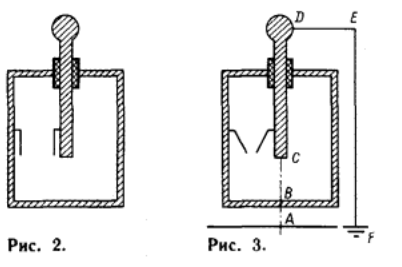
\includegraphics[scale=0.45]{pic2.png}\linebreak
\end{center}

\renewcommand{\arraystretch}{1.5}
\parindent0pt\begin{tabular}[b]{ | m{0.3cm} | m{2.8cm} | m{2.5cm} | m{1.6cm}  | }
\hline
\scriptsize{№} & \scriptsize{\text{Физическая величина}} & \scriptsize{\text{Единица измерения}} & \scriptsize{Обозначения} \\ \hline

\end{tabular}

\parindent72pt
\indent Основные единицы \\

\renewcommand{\arraystretch}{1.5}
\parindent0pt\begin{tabular}[b]{ | m{0.3cm} | m{2.8cm} | m{2.5cm} | m{1.6cm}  | }

\cellcolor{green} \color{white} \text{1} & \cellcolor{green} \color{white} \scriptsize{\text{Длина}} & \cellcolor{green} \color{white} \scriptsize{\text{сантиметр}} & \cellcolor{green}\color{white} \scriptsize{см} \\
\cellcolor{red} \color{yellow} \text{2} & \cellcolor{red} \color{yellow} \scriptsize{\text{Масса}} & \cellcolor{red} \color{yellow} \scriptsize{\text{грамм}} & \cellcolor{red} \color{yellow} \scriptsize{г} \\
\cellcolor{green} \color{white} \text{3} & \cellcolor{green} \color{white}  \scriptsize{\text{Время}} & \cellcolor{green} \color{white}  \scriptsize{\text{секунда}} & \cellcolor{green} \color{white}  \scriptsize{с} \\
\cellcolor{red} \color{yellow} \text{4} & \cellcolor{red} \color{yellow} \scriptsize{\text{Сила}} & \cellcolor{red} \color{yellow} \scriptsize{\text{дина}} & \cellcolor{red} \color{yellow} \scriptsize{дин} \\
%\text{3} & \scriptsize{\text{Давление}} & \scriptsize{\text{дина на $cm^2$}} & \scriptsize{дин/$cm^2$} \\
%\text{3} & \scriptsize{\text{Работа, энергия}} & \scriptsize{\text{эрг}} & \scriptsize{эрг} \\

\end{tabular}
\renewcommand{\arraystretch}{1}

\end{justify}
\end{small}
\end{multicols}
\end{document}
